\documentclass{beamer}
\usepackage[utf8]{inputenc}
\usepackage[T1]{fontenc}
\usepackage[brazilian]{babel}
\usepackage{graphicx}
\usepackage{caption}

\graphicspath{{./imgs/}}
\setbeamertemplate{caption}[numbered]

\usetheme{Warsaw}
\usecolortheme{default}

\title{Apresentação} 
\author[Paulo Pinheiro]
{Dr. Paulo Pinheiro\inst{1}}
\institute[UNIFAP]
{
    \inst{1}
    Centro Universitário Paraíso do Ceará\\
    UNIFAP
}

\date{Última atualização:\\ \today}
\logo{\large \LaTeX{}}
\logo{
\includegraphics[height=0.8cm]{UNIFAP.png}}
%
\begin{document}
% Title page frame
\begin{frame}
    \titlepage 
\end{frame}
% Remove logo from the next slides
\logo{}

%--------------------  FRAMES  ------------------------
%%
% Lists frame
\section{Apresentação}
\subsection{Formação}
\begin{frame}{Formação}
    \begin{columns}[T] % align columns
        \begin{column}{.7\textwidth}
            \textbf{Formação Acadêmica}
            \begin{itemize}
                \item Ms. e Dr. em Eng. de Teleinformática
                \item Bacharel em Física
                \item Graduando em Eng. da Computação
            \end{itemize}
            %
            \vspace{0.2cm}
            %
            \textbf{Atuação Acadêmica}
            \begin{itemize}
                \item Professor de ensino superior de cursos de Engenharia e TI
                \item Instrutor de cursos técnicos nas áreas de TI e elétrica
                \item Gerente de projetos e inovação
            \end{itemize}
        \end{column}%
        %
        \hfill%
        %
        \begin{column}{.35\textwidth}
            \begin{figure}[t!]
                \centering
                \caption{Quase atual.}
                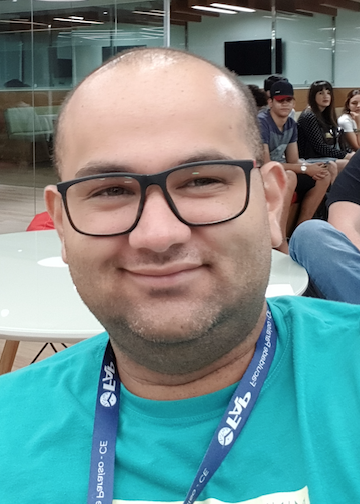
\includegraphics[scale=0.4]{face.png}
                \label{fig:me1}
            \end{figure}
        \end{column}%
    \end{columns}
\end{frame}
%%
\subsection{Pesquisa}
\begin{frame}{Pesquisa acadêmica}
    \begin{columns}[T] % align columns
        \begin{column}{.1\textwidth}
            \begin{figure}[h!]
                \centering
                
\includegraphics[scale=0.2]{pesq.png}
            \end{figure}
        \end{column}%
        %
        \hfill%
        \hspace{0.2cm}
        %
        \begin{column}{.85\textwidth}
            \textbf{Temas de pesquisa acadêmica}
            \begin{itemize}
                \item<1-> [+] PESQUISA DE BASE 
                \begin{itemize}
                    \item [$\star$] Computação quântica e suas nuances.
                    \item [$\star$] Teoria da informação quântica.
                    \item [$\star$] Sistemas ópticos fibrados e free-space.
                    \item [$\star$] Espionagem quântica.
                \end{itemize}
                \item<1-> [+] [EM APERFEIÇOAMENTO]
                \begin{itemize}
                    \item [$\dagger$] Sistemas embarcados.
                    \item [$\dagger$] Arduino e raspberry Pi.
                    \item [$\dagger$] Esp32, Esp8266 NodeMCU e microprocessadores.
                    \item [$\dagger$] IoT - Internet das coisas.
                    \item [$\dagger$] IA aplicada a informação quântica
                \end{itemize} 
            \end{itemize}
        \end{column}
    \end{columns}
\end{frame}
%%
\section{Disciplinas}
\subsection{Disciplinas}
\begin{frame}{Disciplinas}
    \textbf{Disciplinas ministradas}
        \begin{itemize}
            \item [=] Física 1$^*$, 2 e 3. Eletricidade e Eletrotécnica$^*$;
            \item [=] Automação industrial$^*$, Sistemas de controle e digitais.
            \item [=] Telecomunicação e sistemas telefônicos
            \item [=] Lógica de programação e Lógica Matemática$^*$
            \item [=] Sistemas computacionais aplicados
            \item [=] Redes de computadores e sistemas operacionais OFFICE.
            \item [=] Operação de computadores.
            \item [=] Introdução à programação em backend e banco de dados.
        \end{itemize}
        * disciplinas atualmente ministradas.
\end{frame}
%
\subsection{Informações}
\begin{frame}{Informações das disciplinas}
    \begin{block}<1->{Grupos das disciplinas}
        
    \end{block}
    \vspace{0.2cm}
    \begin{block}<2->{Google drive das disciplinas}
        
    \end{block}
\end{frame}
%
\subsection{Contatos}
\begin{frame}{Contatos}
    \begin{block}<1->{Info}
        \begin{itemize}
            \item [$\star$] \textbf{E-mail profissional:} paulo.pinheiro@fapce.edu.br\\
            \item [$\star$] \textbf{E-mail pessoal:} paulovpp@gmail.com\\
            \item [$\star$] \textbf{Linkedin:} https://linkedin.com/in/paulovpp\\
            \item [$\star$] \textbf{GitHub:} https://github.com/paulovpp\\
            \item [$\star$] \textbf{WhatsApp:} +55 88 9 9723-6607
        \end{itemize}
    \end{block}
\end{frame}

% \begin{frame}

% This is an unordered list:
% \begin{itemize}
%     \item Item 1
%     \item Item 2
%     \item Item 3
% \end{itemize}

% and this is an ordered list:
% \begin{enumerate}
%     \item Item 1
%     \item Item 2
%     \item Item 3
% \end{enumerate}

% \end{frame}


% % Blocks frame
% \section{Blocks in Beamer}
% \begin{frame}{Blocks in Beamer}
%     \begin{block}{Standard Block}
%         This is a standard block.
%     \end{block}
%     \begin{alertblock}{Alert Message}
%         This block presents alert message.
%     \end{alertblock}
%     \begin{exampleblock}{An example of typesetting tool}
%         Example: MS Word, \LaTeX{}
%     \end{exampleblock}
% \end{frame} 

\end{document}